\documentclass[german,10pt,a4paper,notitlepage,twocolumn]{article}

\usepackage[hidelinks]{hyperref}
% \usepackage{fancyhdr}
\usepackage{fontspec}
\usepackage[ngerman]{babel}
\usepackage[backend=biber,style=numeric]{biblatex}
\usepackage{graphicx}
\usepackage{float}
\usepackage{amsmath}
\usepackage{amsfonts}
\usepackage{commath}
\usepackage{gensymb}
\usepackage{siunitx}
\usepackage{wallpaper}
\setcounter{secnumdepth}{3}
\setcounter{tocdepth}{3}

\makeatletter
\def\@maketitle{%
  \newpage
  %\null%ORIGINAL
  %\vskip 2em%ORIGINAL
  \begin{center}%
  \let \footnote \thanks
    {\Large\@title \par}%ORIGINAL: \LARGE
    \vskip 0.3em%NEW
    %\vskip 1.5em%ORIGINAL
    {\large
      \lineskip .5em%
      \begin{tabular}[t]{c}%
        \@author
      \end{tabular}\par}%
    \vskip 0.3em%NEW
    %\vskip 1em%ORIGINAL
    {\large \@date}%
  \end{center}%
  \par
  \vskip 0.5em%ORIGINAL
  %\vskip 1.5em%ORIGINAL
}
\makeatother

\LLCornerWallPaper{1}{img/flowchart}

\selectlanguage{german}%
% Space savings:
\usepackage[top=1.5cm, left=2.5cm, right=2.5cm, bottom=3cm]{geometry}
\setlength\parindent{0pt}
\usepackage[extreme]{savetrees}
\flushbottom
\raggedbottom
% Mathematica listening
%fancier pararaphs:
\usepackage{titlesec}
\titleformat{\paragraph}{\normalfont\normalsize\bfseries}{}{}{}
\titlespacing{\paragraph}{0pt}{1em}{0pt}

%hack
\setcounter{tocdepth}{10}

\addbibresource{bib.bib}

\title{\small{Handout}\\Akustische Richtungsbestimmung}
\author{Robin Heinemann\\Jaro Habiger}

\begin{document}
\maketitle
\pagenumbering{gobble}
\section*{Weiterentwicklung seit dem Landeswettbewerb}
Seit dem Landeswettbewerb von Jugend forscht im April haben wir verschiedene Verbesserungen unserers Mikrofonarrays vorgenommen. Der einzige Kritikpunkt der Landesjury war die Unhandlichkeit unseres Mikrofonarrays. Deshalb haben wir das Mikrofonarray miniaturisiert. Zusätzlich dazu haben wir die Anpassungsfähigkeit an dynamische Lautstärke verbessert.
\subsection*{Miniaturisierung}
Bei unserem alten Mikrofonarray war der hauptsächliche Grund für die Größe die Länge der Mikrofone. Außerdem waren wir an die auf dem Markt üblichen Audiointerfaces gebunden und dadurch stark begrenzt in der Funktion und Umsetzung unseres Mikrofonarrays.
\subsubsection*{Digitale MEMS Mikrofone}
Eine Alternative zu den herkömmlichen Messmikrofonen, die wir vorher verwendet haben, stellen MEMS Mikrofone dar. Diese können sehr klein und billig hergestellt werden, da auf bestehende Herstellungsprozesse der Halbleitertechnik zurückgegriffen werden kann. Eine Unterkategorie der MEMS Mikrofone sind die digitalen MEMS Mikrofone. Bei diesen wird der Prozess der Digitalisierung schon im Mikrofon vorgenommen. Also wird ein Teil der Aufgabe des Audiointerfaces vom Mikrofon übernommen. Das Mikrofon sendet einen digitalen Datenstrom (in unserem Fall \textit{i$^2$s}).
\begin{figure}[H]
    \centering
    \includegraphics[width=\linewidth]{img/SMD3}
    \vspace{-2em}
    \caption{Vergrößerte Aufnahme eines MEMS Mikrofons}
    \label{fig:mems}
\end{figure}
\subsubsection*{Spezielle Hardware}
Da die von uns verwendeten MEMS Mikrofone sehr viele Anschlüsse auf sehr kleinem Raum haben, waren speziell angefertigte Platinen notwendig. Besonders an unserem Mikrofonarray ist auch, dass es komplett aus Platinenmaterial besteht, woraus sich bedeutende Vorteile bei Produktion und Handhabung ergeben.
\begin{figure}[H]
    \centering
    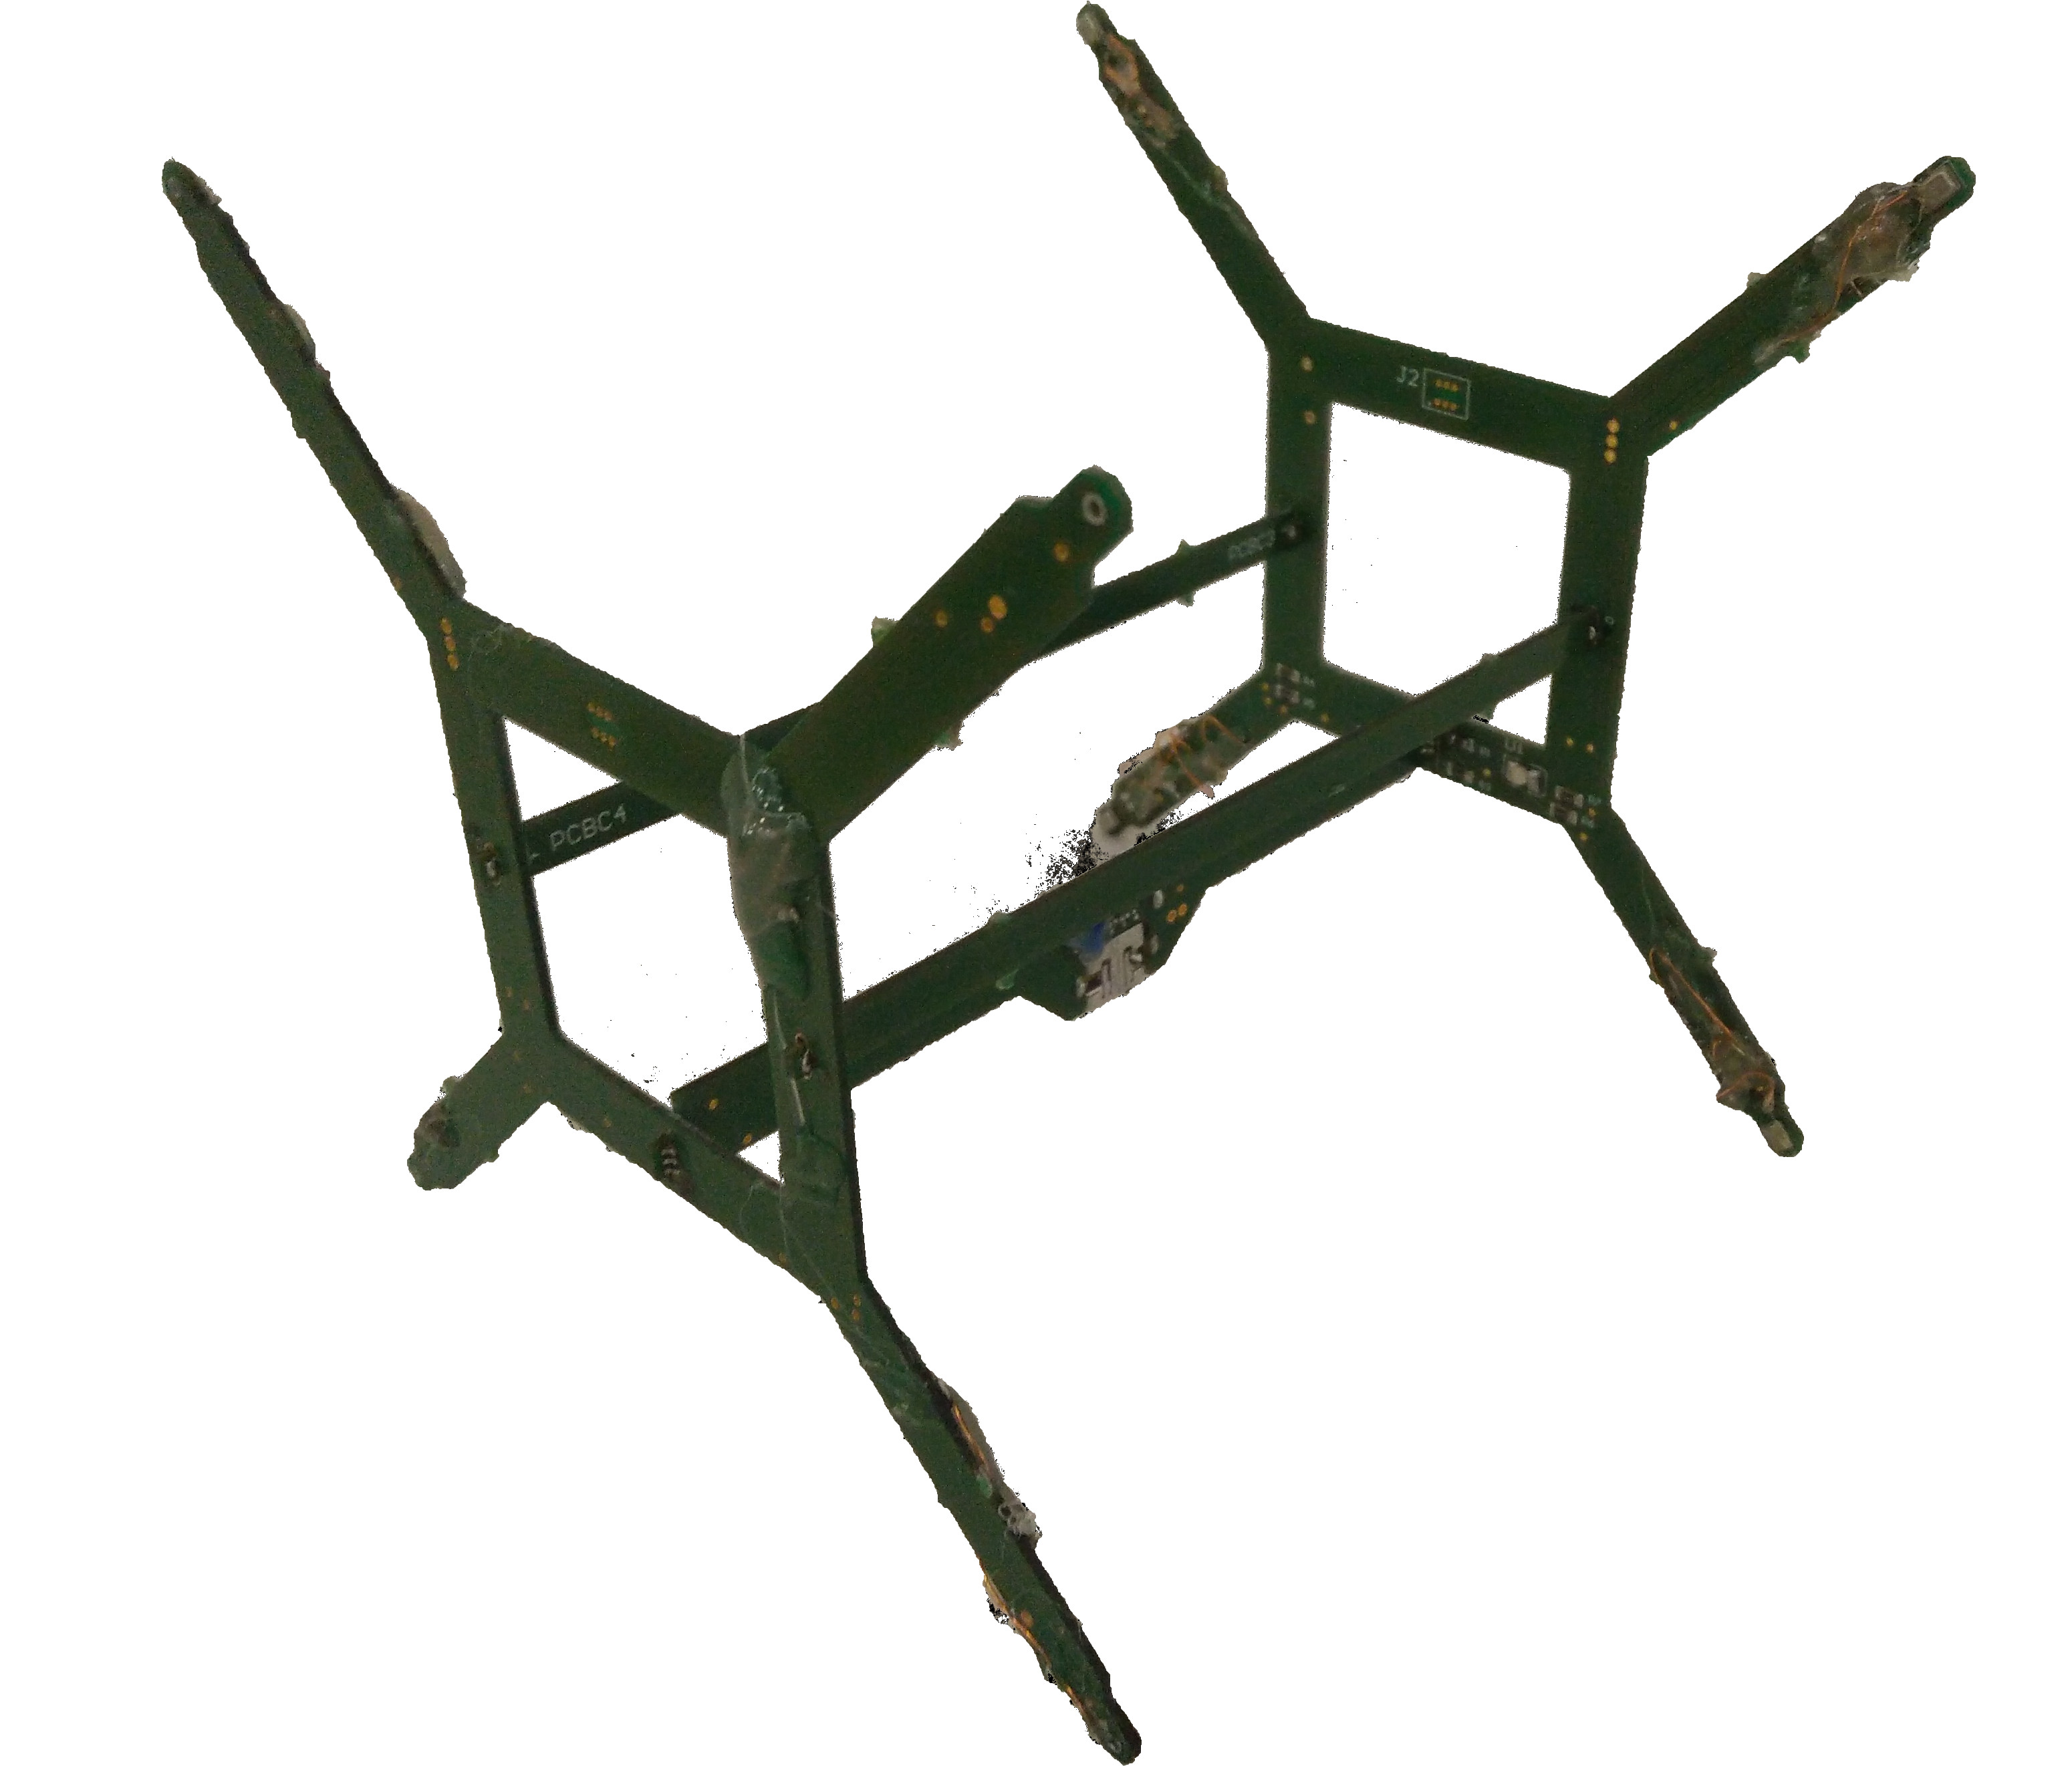
\includegraphics[width=\linewidth]{img/cube}
    \vspace{-2em}
    \caption{Foto unseres neuen Mikrofonarrays}
    \label{fig:cube}
\end{figure}
\subsubsection*{Ersetzen des Audiointerfaces}
Um die \textit{i$^2$s} Signale, die von dem Mikrofon ausgesendet werden, einzulesen, und in die bestehende Verarbeitungskette unseres Verfahrens zu integrien, mussten diese in einen Netzwerkdatenstrom ungewandelt werden. Hierfür haben wir einen \textit{FPGA SoC} verwendet. Das \textit{FPGA} Design haben wir mit der Hardwarebeschreibungssprache \textit{VHDL} entwickelt. Zusätzlich haben wir einen Treiber für Linux geschrieben, der die Daten vom \textit{FPGA} weiterleitet. Die Kombination aus Gerätetreiber und \textit{FPGA} ersetzt also zusammen mit dem \textit{ADC} im Mikrofon das komplette Audiointerface.
\subsection*{Dynamische Lautstärkeanpassung}
Ein weiteres Problem, das uns während der Evaluation unseres neuen Mikrofonarrays aufgefallen ist, ist die hohe Dynamik der Lautstärke in einer typischen Anwendungssituation. Um diese auszugleichen, haben wir ein Modul entwickelt, das die Verstärkung der Tonaufnahme an die Umgebungslautstärke anpasst.
\subsection*{Fazit}
Durch die Verwendung modernster Digitaltechnik konnten wir die Anregungen der Landesjury umsetzten und die Anwendbarkeit unseres Verfahrens verbessern.
\vspace{-100pt}
\end{document}
